\chapter{LAPD Simulation Details}
\label{c_lapd_sim}

I simulate the model equations using the BOUT++ code~\cite{dudson2009}, which I describe in Appendix~\ref{app_bout}. 
There I discuss the nitty gritty aspects of the code and the specific numerical routines that
I use. Otherwise, the programming and numerical details are hidden so that I may focus on the physics model and the physics results in the main text.

In this chapter then, I state and explain the equations, boundary conditions, parameters, and profiles that I use in the LAPD simulations. 
In all of the simulations hence forth (except for in Appendix~\ref{app_mean_flow}), I use the same equations, parameters and profiles. I change only the axial boundary conditions between simulations,
which I will specifically discuss in Sec.~\ref{s_bcs}. 
Overall, however, I concentrate on replicating through simulation one particular LAPD experiment and fully analyzing it. This precludes the exploration of
parameter scalings but allows me to deeply consider the underlying physics of a particular turbulent system. So this chapter details the model that I use to simulate and study that system.

\section{The Equations}
\label{s_equations}

I use the Braginskii equations as shown in Chapter~\ref{c_braginskii} to model LAPD turbulence. I separate all variables into time-independent equilibrium parts and time-dependent
fluctuating parts so that I may use experimental time-independent profiles as input. The alternative would be to solve the full equations with no equilibrium/fluctuation separation
and no experimental profile input. The difficulty in this alternative technique is the need to specify sources, sinks, and boundary conditions, which can be difficult to measure or estimate.
This alternative method has been untertaken by Rogers and Ricci~\cite{rogers2010}. My approach is easier to implement, and since the time-independent profiles are so important in driving the turbulence,
I feel that inputing the experimentally measured profiles can help produce physically realistic turbulence.

Because of my equilibrium/fluctuation separation technique, I can linearize the equations, keeping only one nonlinearity in each equation: the
advective nonlinearity. While this isn't necessary, it does simplify the energy dynamics as formulated in Chapter~\ref{c_en_formalism}. The justification is practical rather than mathematical,
and the partially linearized equations produce fluctuations that are quite statistically similar to experimental fluctuations, which is shown in Chapter~\ref{c_lapd_turb}, so I feel justified
in doing this.

In the equations below, I normalize all quantities to give dimensionless variables. All times are normalized to the inverse ion cyclotron frequency $\omega_{ci} = \frac{e B}{m_i}$, 
velocities are normalized to the ion sound speed $c_s = \sqrt{\frac{T_e}{m_i}}$, lengths are normalized to the sound gyro-radius $\rho_s = c_s/\omega_{ci}$, potentials to $T_e/e$,
densities to the density at the radial cylindrical axis, and temperatures to the temperature at the cylindrical axis. 
Quantities such as $c_s$ that are typically functions of radius due to the radial dependence of
the electron temperature are taken to be constant in these normalizations, where I use the values at the radial axis. The equations below don't reflect this, but the transport coefficients
in the actual code do. So, the LAPD simulation equations are as follows:

\beqar
\label{ni_eq}
\pdt N = - {\mathbf v_E} \cdot \grad N_0 - N_0 \gradpar \vpe + \mu_N \gradperp^2 N + S_N + \{\phi,N\}, \\
\label{ve_eq}
\pdt \vpe = - \fmie \frac{T_{e0}}{N_0} \gradpar N - 1.71 \fmie \gradpar T_e  + \fmie \gradpar \phi - \nue \vpe + \{\phi,\vpe \}, \\
\label{rho_eq}
\pdt \varpi = - N_0 \gradpar \vpe  - \nuin \varpi + \mu_\phi \gradperp^2 \varpi + \{\phi,\varpi \}, \\
\label{te_eq}
\pdt T_e = - {\mathbf v_E} \cdot \grad T_{e0} - 1.71 \frac{2}{3} T_{e0} \gradpar \vpe + \frac{2}{3 N_0} \kpe \gradpar^2 T_e  \nonumber \\
- \frac{2 m_e}{m_i} \nue T_e  + \mu_T \gradperp^2 T_e +  S_T + \{\phi,T_e\}.
\eeqar

Note that the advective nonlinearities in each equation are written with Poisson brackets. Additionally, the only equilibrium profiles are $N_0$ and $T_{e0}$, which are only functions of radius.
$\phi_0 = v_{\parallel e 0} = 0$ in these equations. The linearized vorticity is $\varpi = \gradperp \cdot (N_0 \gradperp \phi)$. $N, \vpe, \phi,$ and $T_e$ are fluctuating first-order quantities.

These equations have a few additional terms not included in the equations of Chapter~\ref{c_braginskii}. First, I have included density and temperature sources $S_N$ and $S_T$. I have left out
a momentum source as well as the contribution of the density source to changes of the momentum and temperature. Second, I have included diffusive ($\mu_N \gradperp^2 N$ and $\mu_T \gradperp^2 T_e$) 
and viscous ($\mu_\phi \gradperp^2 \varpi$) terms in Eqs.~\ref{ni_eq}, ~\ref{te_eq}, and~\ref{rho_eq} respectively.

\subsection{Sources}
\label{ss_sources}

The density source is actually a source/sink. It models both the ionization of neutral atoms as well as the recombination of ions and electrons. The sink action in LAPD
is dominated by parallel (along ${\bf B}$) losses to materials at the machine ends because the magnetic field prevents rapid radial loss. 
It's also possible that a layer of neutral atoms near the end of
the machine opposite the cathode cools the plasma enough so that recombination can be strong in this layer. The sink action occurs at all radii with finite plasma density, which constitutes regions
both inside and outside of the cathode radius due to radial ion transport. If the sink action is primarily at the end plates, the sink can be calculated by $2 n_{se} c_s/L_{\para}$, where
$n_{se}$ is the density at the sheath edge in front of the end plate, $c_s$ is the sound speed at the sheath edge, and the factor of 2 accounts for the two plates. $n_{se}$ and $c_s$ are functions
of radius such that the sink is strongest at the radial axis and decreases at larger radii. Calculation of the sink term requires knowledge of the density and temperature at the end of the machine,
which is generally not measured experimentally.

The ionization source occurs primarily inside of the cathode radius. The source term is calculated with $n_e n_n \left<\sigma v \right>_{iz}$, 
where $n_n$ is the neutral Helium density and $\left< \sigma v \right>_{iz}$
is the ionization rate of Helium and is a strong function of temperature. The strong temperature dependence is the reason why ionization occurs only within the cathode radius.
Ionization rates are readily available~\cite{stangeby2000}, but the neutral density is not, making the source difficult to calculate. However, it is clear that if one were to sum up
the source and sink and integrate axially, the region inside of the cathode radius must be a net source, while the region outside of it must be a net sink.

Now when I simulate the turbulence in LAPD without the source terms, turbulence drives radial transport such that the total flux-surface-averaged density gradient relaxes over time as seen
in Fig.~\ref{source} a) until the radial transport ceases. It's interesting that $\left< N_t \right>_{fs} = \left< N_0 + N \right>_{fs}$ doesn't become totally flat, but maintains a gradient. 
This is probably a result of the turbulence transport ceasing and the
partial linearization of the equations, specifically the diffusion term $\mu_N \gradperp^2 N$, preventing classical transport of the total equilibrium profile. Also the radial boundary conditions
probably have an affect as well. Nevertheless, the strong relaxation that is present is not physical because of the experimentally present source/sink mechanism. 

\begin{figure}[!ht]
\centerline{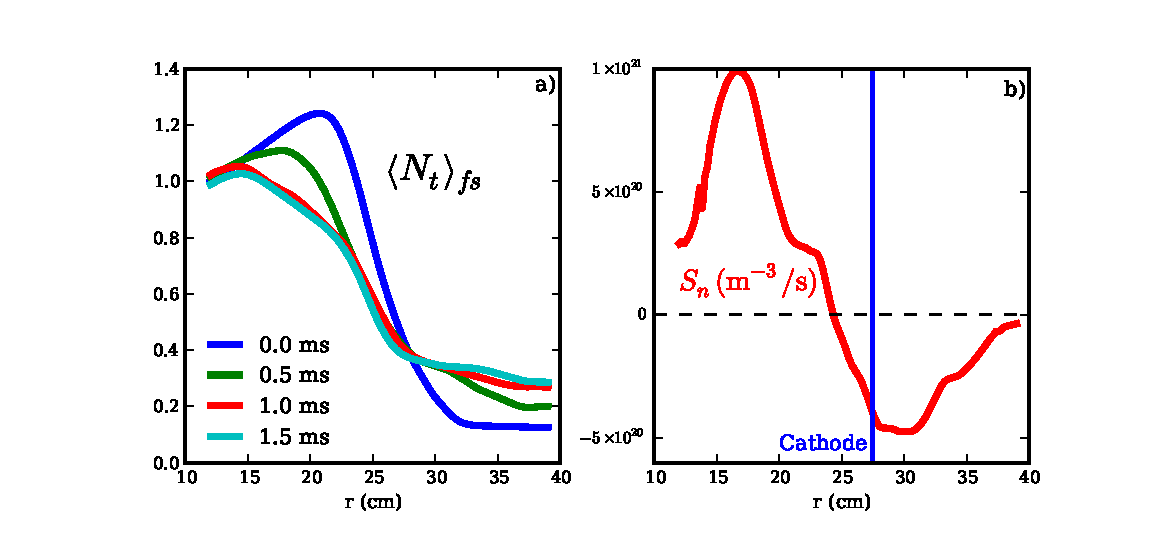
\includegraphics[]{source}}
\caption{Profile relaxation and evolved density source}
\label{source}
\end{figure}


Now, rather than developing a first principle's source based on the theoretical source/sink expressions, I use ad hoc controlling sources. 
I estimate that $\left< N_t \right>_{fs}$ remains relatively constant over time, and model the source using the integral
portion of a PID controller. This means that I write an equation for the source:

\beq
\label{Sn_eq}
\pdt{S_n} = - \left< N \right>_{fs}.
\eeq

Therefore,

\beq
\label{Sn_eq2}
S_n(t) = - \int_0^t \left< N(\tau) \right>_{fs} d\tau.
\eeq

A typical time-averaged density source is shown in Fig.~\ref{source} b).
The upshot of using such a source is that $\left< N_t(t) \right>_{fs} \simeq N_0$. Notice that the source in Fig.~\ref{source} b) is net positive inside of the cathode radius and negative
outside of it, just as one would expect.
I use the same method for the temperature source. The temperature source ultimately comes from the hot electrons that are boiled off of
the cathode, which transfer their energy to the plasma through ionizing collisions. This heat transfer is mostly to the electrons of the plasma. The temperature sink is caused by collisions
with ions and neutrals which line radiate and by heat loss to the sheath and end walls.

I emphasize that the sources are not first principle sources. They are constructed based on the simulated radial transport. The alternative first principle's approach was used by Rogers and Ricci
for LAPD~\cite{rogers2010}. They use a stationary top-hat-like ionization source that models the physical density-producing process in LAPD. 
Furthermore, they do not separate equilibrium from fluctuations or input equilibrium profiles. Their source feeds the density, which then transports itself until it comes to a quasi-equilibrium state
(a sink is also present). This method solves for the full plasma state with very little experimental input. 
They input the sources and derive the plasma state. On the other hand, I input part of the plasma
state and derive the sources. As stated before, our method has the advantage of using experimentally measured profiles. 
This experimental input allows us to more easily simulate turbulence that resembles that
in the experiment, and therefore make conclusions on the fluctuation properties. I do not, however, evolve the equilibrium and gain the knowledge that comes from that.

Before I go on, I note that in the past, Pavel Popovich and I tried a number of different approaches to the source problem. One approach was simply to remove the flux-surface-averaged fluctuating
density and temperature components at each time step. This is similar to the source technique above, but it supplies a quicker cutoff of the flux-surface-averaged fluctuating components than the
source above because it doesn't preserve past history of the source. Another technique that we used was to derive a source like that in Fig.~\ref{source} b) in one simulation, and then start
another simulation using that as a purely time-independent source. This supplied a slower cutoff of the flux-surface-averaged fluctuating components than the other two methods. Results of
the evolution of the total density profile can be seen in Popovich et al.~\cite{popovich2010b}. In any case, we couldn't find any significant difference in the results upon use of these different
sources. This third technique is just too slow to implement, so I do not use it for simulations in this paper. I prefer the PID source in general. Furthermore, I generally implement a condition
with the PID source so that it does not drive the total density or temperature negative as I discuss in Appendix~\ref{app_bout}.

\subsection{Artificial Diffusion and Viscosity}
\label{ss_art_diff}

Artificial diffusion or hyperdiffusion terms are ubiquitous in fluid simulations. They are generally intended to prevent high frequency or high wavenumber ringing caused by numerical advection
schemes at steep interfaces. They can, however, cause unphysical smoothing in systems that are non-diffusive and non-viscous or cause over-smoothing if applied haphazardly. Some numerical
advection schemes contain their own diffusion, called numerical diffusion. Other non-advective finite difference schemes also contain numerical diffusion or dispersion.

I use artificial diffusion and viscosity for several reasons. The first is to prevent artificial high-wavenumber oscillations due to the Arakawa advection scheme that I use~\cite{arakawa1966}.
Second, it smooths out the solutions, preventing the total density and temperature from becoming negative at any point in space, which is obviously unphysical. Third, I can use it
to prevent the need to go to very fine grid spacing at which physical diffusion and viscosity are important. Finally, I can use it to help saturate the turbulence at levels consistent with experiment.
These reasons are all somewhat related, and I note that I performed an artificial diffusion and viscosity sensitivity study in Ref.~\cite{friedman2012}.

Diffusion and viscosity are real effects that are present in the non-reduced Braginskii equations. In Chapter~\ref{c_braginskii}, I made the approximation that 
$\grad \cdot (n {\bf v}_{\perp e}) = {\bf v}_{E} \cdot \grad n$, which neglected the polarization velocity part of ${\bf v}_{\perp e}$. Now the ``full polarization velocity''~\cite{simakov2003}
(from crossing Eq.~\ref{brag_mom} with ${\bf b}$ and neglecting the stress tensor) is

\beq
\label{e_pol_v}
{\bf v}_{p e} = (1/\omega_{ce}) \left[  \diff{({\bf b \times v}_{\perp e})}{t} + \nue {\bf b \times v}_{\perp e} - \nue {\bf b \times v}_{\perp i} - \frac{3}{2} \frac{\nue}{m_e \omega_{ce}} \gradperp T_e  \right].
\eeq

The part of this that causes collisional diffusive terms is $ (\nue/\omega_{ce}) {\bf b \times v}_{\perp e}$. Now this contains ${\bf v}_{\perp e}$ itself, which must be approximated as 
${\bf v}_{\perp e} = {\bf v}_{E} + {\bf v}_{d e}$ to allow for closure. Only the diamagnetic drift part will be important for the collisional diffusion, so the part of the polarization velocity that I
focus on is $(\nue/\omega_{ce}) {\bf b \times v}_{d e}$. Recall that I want to use this in the continuity equation, so I am interested in the term 
$\grad \cdot (n_e v_e) \rightarrow \grad \cdot \left( n_e (\nue/\omega_{ce}) {\bf b \times v}_{d e} \right) = - \grad \cdot \frac{\nue m_e}{e^2 B^2} \gradperp p_e$. Now defining 
$D = \frac{\nue m_e T_e}{e^2 B^2}$, I have $\grad \cdot (n_e v_e) = - \grad \cdot (D \gradperp n) +$ lots of other terms. $D$ is the classical diffusion coefficient, which is about $0.01 {\rm m^2/s}$
for LAPD parameters. One of the terms in $\grad \cdot (D \gradperp n)$ is $D \gradperp^2 n$, which has the same form of the artificial diffusion term that I've added to Eq.~\ref{ni_eq}. 
Of course, I have neglected many terms of the same order as this term in Eq.~\ref{ni_eq}, but this shows that such a classical diffusion term is present in the Braginskii equations.

A similar treatment can be used for the energy conservation equation (Eq.~\ref{brag_ener}), using the same procedure as for the continuity equation but with the $p_e \grad \cdot {\bf v}_e$ term in
Eq.~\ref{brag_ener}. The result is $p_e \grad \cdot {\bf v}_e = D n_e \gradperp^2 T_e +$ lots of other terms. This has the same form as the temperature diffusion term in Eq.~\ref{te_eq}.

The viscosity in the vorticity equation comes from the ion stress tensor term $\pdiff{\Pi_{i \alpha \beta}}{x_\beta}$ 
that I neglected when deriving the vorticity equation because I neglected everything with finite
ion temperature. If this was included, a vorticity diffusion term (aka a viscosity) would have been included in the vorticity equation~\cite{popovich2010b}
as it is in other equation sets like the well-known Hasagawa-Wakatani equations~\cite{hasegawa1983}. 
The magnetized Braginskii viscosity coefficient is $\eta_1^i = \frac{3 n T_i}{10 \omega_{ci}^2 \tau_i}$, which is about $2 \times 10^{-8} { \rm kg/m \cdot s}$ 
for LAPD. Since LAPD's ions are not necessarily magnetized due to the fact that $\omega_{ci} \tau_i \sim 1$, the unmagnetized ion viscosity is $\eta_0^i = 0.96 n T_i \tau_i$~\cite{Braginskii1965}
which is about $4 \times 10^{-7} {\rm kg/m \cdot s}$.

For the artificial diffusion and viscosity coefficients in Eqs.~\ref{ni_eq}-\ref{te_eq}, I use a single value of $1.25 \times 10^{-3}$ in our normalized units, 
which is $0.075 {\rm m^2/s}$ in real units.
I find that this value produces turbulent fluctuation levels consistent with experimental levels. 
I use this as a free parameter in this sense. This value is much larger than the real classical diffusion $D$,
but is smaller than $\frac{\eta_1^i}{n m_i} = 1 {\rm m^2/s}$. 
Nevertheless, I neglected a number of terms in Eqs.~\ref{ni_eq}-\ref{te_eq} such that there isn't justification to use the real diffusion and 
viscosity in these equations. Artificial diffusion and viscosity terms, however, serve a numerical purpose.


\section{Boundary Conditions}
\label{s_bcs}

Boundary conditions are often difficult to determine in plasma devices. While the properties of the boundaries are usually known, the way that the plasma interacts with them can be complex.
Plasma boundary physics is one of the main elements of present day fusion research~\cite{stangeby2000}. Often times there is uncertainty in the equations that need to be used in simulations,
and once the equations are found, they can be difficult to implement in codes.

The boundary conditions in LAPD are difficult to determine. LAPD contains at one end, a hot emitting cathode behind a biased mesh annode. In front of the annode are biasable azimuthal limiters
with radius about equal to the cathode radius, though the limiter radius may be changed. The far end contains a floating mesh plate. The cylinder is conducting and has a radius about 20 cm larger
than the cathode radius.

\subsection{Simple Boundaries}
\label{ss_s_bc}

In all simulations, I use an annulus rather than a cylinder. Although the inner radius of the annulus may be arbitrarily small, I take the inner radius to be 12 cm. I take the outer radius
to be 39 cm. This is generally the radial extent of our experimental probe measurements. Furthermore, the plasma fluctuations are nearly zero (when normalized to values at the cylindrical axis)
outside of this annular
region, which is seen in Fig.~\ref{es_vs_em_stats} c). Therefore, I set the radial boundaries on all of the fluctuating variables ($N, \phi, \vpe, {\rm and } T_e$) to zero. It would be nice
in the future to take data spanning at least a few more cm and extend the simulation domain accordingly. But for now, the results use such an annular domain.

As for the axial boundaries, I use four different boundary conditions: periodic, zero-value (Dirichlet), zero-derivative (Neumann), and Bohm sheath. 
The only non-trivial one, Bohm sheath, is derived and described in
the following subsection. The others are all trivial to implement and provide a test of the importance of the axial boundary conditions on the nature of the turbulence.

\subsection{Bohm Sheath Boundaries}
\label{ss_bs_bc}

Bohm sheath boundary conditions are applicable when a plasma terminates at a conducting plate. I note that this is not necessarily the case in LAPD. 
The cathode/annode system is obviously much different from a simple floating or biased conducting plate. Furthermore, the mesh wall at the far end is not a solid wall.
Moreover, it's not clear if the plasma is even attached to the far end mesh wall or if it becomes detached in the neutrals in front of it, where the plasma cools and recombines
before interacting with the wall. In any case, it is still instructive to apply such an idealized boundary condition to LAPD because it is somewhat more realistic
than the simpler boundary conditions, and it creates a new linear instability (see Sec.~\ref{ss_cwm}), which can be used to test the robustness of LAPD's nonlinear instability.
Therefore, I proceed with the derivation of the Bohm sheath boundary conditions.

Now, it is known that to good approximation, a plasma bounded by a wall can be divided into two regions: the main plasma and the Debye sheath~\cite{stangeby2000}. 
The Debye sheath is a small region adjacent to the wall, generally several Debye lengths long. It has a net positive charge ($n_i > n_e$) 
that shields the negative charge on the wall. The sheath does not completely shield the negative wall, however, and a small electric field penetrates into
the main plasma (the ambipolar field), which mostly serves to accelerate the cold ions toward the wall, and slightly retard the electrons before entering the sheath.
In the main plasma, the quasi-neutrality relation holds ($n_i = n_e$). 

The well-known Bohm criterion along with other considerations restricts the ions to move into the sheath entrance at the sound speed $c_s = \sqrt{T_e/m_i}$. 
I consider here the case where there is no external biasing; in other words, the end plates are electrically isolated and floating.
The wall can be set to an arbitrary potential, say $\phi_w = 0$, while the potential at the sheath entrance is then the positive 
floating potential $\phi_{sf}$. This potential difference across the sheath reflects slow electrons that enter the sheath.
The electrons approximately maintain a cutoff Maxwellian velocity distrubution throughout the sheath, and at the wall, 
their velocity is retarded by a Boltzmann factor due to the floating potential. 
In total, the current to the wall is~\cite{berk1991,berk1993,xu1993}

\beq
\label{sheath_current}
J_\parallel = \pm e n \left [ c_s - \frac{(T_e/m_e)^{1/2}}{2 \sqrt{\pi}} e^{\left(- \frac{ e \phi_{sf}}{T_e}\right)} \right ],
\eeq

where the $\pm$ indicates that the plasma flux goes into the wall, which is in different directions for the different end plates.
Note that there is a factor of $\sqrt{2}$ discrepancy between different reports on the expression used for the thermal velocity, which should have only a minor consequence.
In this expression, all values are total (equilibrium + fluctuations).

Now, this is not only the current to the wall, but also the current going into the sheath edge, since the sheath is too small for there to be appreciable radial current loss or an ionization source
within the sheath. All values, in fact, are taken to be those at the sheath edge.
Furthermore, since the wall is electrically isolated, the equilibrium current at the wall vanishes.
This sets the value for the floating potential to be $\phi_{sf} = \Lambda T_{e0} / e$ with $\Lambda = {\rm ln} \left(\frac{1}{2 \sqrt{\pi}} \sqrt{\frac{m_i}{m_e}} \right)$.
Note that $T_{e0}$ is a function of radius, meaning $\phi_{sf}$ is also a function of radius. Thus, a radial temperature gradient produces a radial
electric field, at least at the sheath edge and likely penetrating axially into the main plasma. 
It is noted that $J_\parallel$ need not vanish on every field line since the end plates are conducting and charges can move around on the plate, 
however, the vanishing equilibrium current is generally a fair approximation~\cite{berk1993}.

On the other hand, the fluctuating component of the current is allowed to vary between field lines.
The first order fluctuating component is obtained by linearizing Eq.~\ref{sheath_current}, giving the result:

\beq
\label{lin_sheath_current}
J_\parallel = \pm e N_0 c_{s0} \left [ \frac{e \phi}{T_{e0}} - \Lambda \frac{T_e}{T_{e0}} \right ],
\eeq

where now, $J_\para, \phi$ and $T_e$ are fluctuating components, consistent with previous notation.
This expression for the current sets the fluctuating axial boundary condition of the plasma and is often called the Bohm Sheath boundary condition. This current condition holds both at
the wall and at the sheath entrance. So rather than taking the simulation
domain all the way to the wall, simulations often end at the sheath entrance and employ this analytically derived boundary condition to the boundaries of the main plasma. 
Then one doesn't have to worry about the small spatial scales and the non-quasineutrality of the sheath.
The corresponding boundary conditions for the other fluid variables such as the density and temperature have recently been derived by Loizu et al.~\cite{loizu2012}. However, I
simply take them to have zero-gradient as most others have done, although this isn't wholly inconsistent with Loizu's calculations.

Now while one may set the parallel current (or equivalently $\vpe$) at the axial boundaries to the quantity on the right hand side of Eq.~\ref{lin_sheath_current}, I don't do that.
I use Ohm's Law ($- \gradpar \phi = \eta_\para J_\para$) to set the boundary condition for the gradient of $\phi$. I do this for practical reasons in the coding. Therefore, the
boundary condition used in the code is (in our normalized units):

\beq
\label{sheath_bc}
\gradpar \phi = \pm \frac{\nue m_e}{m_i} \left(\phi - \Lambda T_e  \right).
\eeq



\section{Profiles and Parameters}
\label{s_profs_params}

\begin{figure}[!ht]
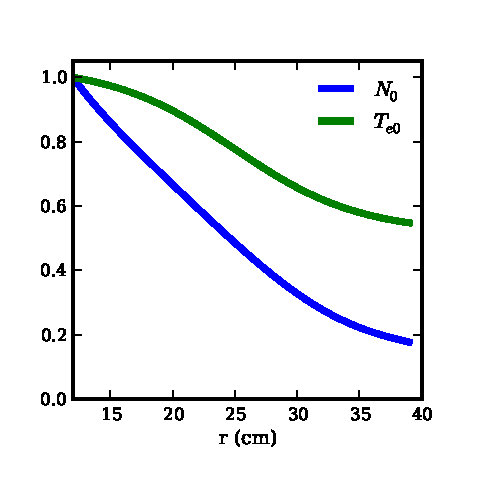
\includegraphics[]{equilibrium_profiles}
\centering
\caption{Equilibrium density and electron temperature profiles}
\label{equilibrium_profiles}
\end{figure}


As explained above, I take all equilibrium profiles and parameters from experimental measurements. 
All simulations use profiles and parameters from one particular experiment.
This experiment used limiter biasing to essentially null out the mean radial electric field~\cite{schaffner2012}. I used this experiment so that I could neglect the mean potential profile
in the equations (as is done in Eqs.~\ref{ni_eq}-\ref{te_eq}), which simplifies our analysis. The normalized profiles that I use are shown in Fig.~\ref{equilibrium_profiles}, and the parameters
are shown in Table~\ref{parameter_table}. The density profile is
a polynomial fit to the experimental equilibrium density profile. The temperature profile is a tanh function that somewhat resembles typical LAPD temperature profiles. At the time of the first
simulations, I didn't have reliable temperature profile measurements, so I was forced to estimate what the profile might look like. I note that the real temperature profile has a steeper
gradient than the one I use. And again, I use $\phi_0 = 0$, which is a good approximation for the experimental nulled out potential profile.

The profiles that I use have no azimuthal or axial variation because I don't have the corresponding experimental measurements. So I assume that the equilibrium profiles are only functions
of radius. It's likely, however, that there is some axial variation in the profiles and parameters. In LAPD, $\nu^* \equiv L_\para/\lambda_{ei} \sim 100$, generally indicating that a
parallel temperature gradient can exist depending on the locations of the sources and sinks~\cite{stangeby2000}. 
Furthermore, if the Bohm sheath boundary condition is correct, the equilibrium potential must have a parallel gradient in order
to accelerate the ions up to the sound speed at the sheath entrance. This ambipolar parallel electric field should exist between the location of the sheath entrance and an ion collision length
into the main plasma. The parallel electric field generated by the condition of Eq.~\ref{sheath_bc} is just the perturbed field that responds to electron temperature perturbations. It doesn't
constitute the equilibrium electric field. 

Moreover, recall that the Bohm sheath condition combined with a radial equilibrium electron temperature profile implies (at least near the sheath) a corresponding equilibrium potential profile, since 
$\phi_{sf} = \Lambda T_{e0} / e$. Experimentally, this relation doesn't hold where the plasma is measured, meaning that either the ambipolar field doesn't penetrate far into the plasma or that
the real LAPD boundary conditions are more complicated than simple floating conducting plates. So I don't use any equilibrium axial variation, leaving this to future work.



\begin{table}
\label{parameter_table}
\setlength{\tabcolsep}{60pt}
\begin{tabular}{| c c |}
\hline \hline
Species & $^4$He \\
$Z$ & $1$ \\
$n$ & $2.86 \times 10^{18}$ m$^{-3}$ \\
$T_e$ & $6$ eV \\
$T_i$ & $\lesssim 1$ eV \\
$B_0$ & $0.1$ T \\
$L_\para$ & $17$ m \\
$a$ & $0.4$ m \\
$\lambda_D$ & $10^{-5}$ m \\
$\omega_{ci}$ & $2.4 \times 10^6$ rad/s \\
$\omega_{ce}$ & $1.8 \times 10^{10}$ rad/s \\
$\rho_e$ & $ 5.3 \times 10^{-5}$ m \\
$\rho_i$ & $\sim 1 \times 10^{-3}$ m \\
$\rho_s$ & $5 \times 10^{-3}$ m \\
$v_{te}$ & $9.4 \times 10^{5}$ m/s \\
$c_s$ & $1.1 \times 10^4$ m/s \\
$v_A$ & $7 \times 10^5$ m/s \\
$\beta$ & $5 \times 10^{-4}$ \\
$m_e/m_i$ & $1.4 \times 10^{-4}$ \\
ln$\Lambda$ & $11$ \\
$\nue$ & $7.2 \times 10^6$ Hz \\
$\lambda_{ei}$ & $0.13$ m \\
$\nu_i$ & $\sim 10^6$ Hz \\
$\nu_{in}$ & $3 \times 10^3$ Hz \\
$\kappa_\para^e$ & $9.8 \times 10^{23}$ eV/m$^2$ s \\
$\eta_0^i$ & $\sim 10^{12}$ eV s/m$^3$ \\
$\omega_{*}$ & $\sim 5 \times 10^4$ rad/s \\
\hline \hline
\end{tabular}
\caption{LAPD simulation parameters}
\end{table}
